% Use only LaTeX2e, calling the article.cls class and 12-point type.

\documentclass[12pt]{article}

% Users of the {thebibliography} environment or BibTeX should use the
% scicite.sty package, downloadable from *Science* at
% www.sciencemag.org/about/authors/prep/TeX_help/ .
% This package should properly format in-text
% reference calls and reference-list numbers.

\usepackage{scicite}

% Use times if you have the font installed; otherwise, comment out the
% following line.

\usepackage{times}

% The preamble here sets up a lot of new/revised commands and
% environments.  It's annoying, but please do *not* try to strip these
% out into a separate .sty file (which could lead to the loss of some
% information when we convert the file to other formats).  Instead, keep
% them in the preamble of your main LaTeX source file.


\usepackage{graphicx}
\usepackage{hyperref}
\usepackage{subcaption}

% The following parameters seem to provide a reasonable page setup.

\topmargin 0.0cm
\oddsidemargin 0.2cm
\textwidth 16cm 
\textheight 21cm
\footskip 1.0cm


%The next command sets up an environment for the abstract to your paper.

\newenvironment{sciabstract}{%
\begin{quote} \bf}
{\end{quote}}


% If your reference list includes text notes as well as references,
% include the following line; otherwise, comment it out.

\renewcommand\refname{References and Notes}

% The following lines set up an environment for the last note in the
% reference list, which commonly includes acknowledgments of funding,
% help, etc.  It's intended for users of BibTeX or the {thebibliography}
% environment.  Users who are hand-coding their references at the end
% using a list environment such as {enumerate} can simply add another
% item at the end, and it will be numbered automatically.

\newcounter{lastnote}
\newenvironment{scilastnote}{%
\setcounter{lastnote}{\value{enumiv}}%
\addtocounter{lastnote}{+1}%
\begin{list}%
{\arabic{lastnote}.}
{\setlength{\leftmargin}{.22in}}
{\setlength{\labelsep}{.5em}}}
{\end{list}}


% Include your paper's title here

\title{Hemoglobin A1c Measurement Impact on Hospital Readmission Rates.} 


% Place the author information here.  Please hand-code the contact
% information and notecalls; do *not* use \footnote commands.  Let the
% author contact information appear immediately below the author names
% as shown.  We would also prefer that you don't change the type-size
% settings shown here.

\author
{Matthieu Marinangeli$^{1}$\\
\\
\normalsize{$^{1}$\'Ecole Polytechnique F\'ed\'erale de Lausanne (EPFL), Switzerland}\\
\\
}

% Include the date command, but leave its argument blank.

\date{}



%%%%%%%%%%%%%%%%% END OF PREAMBLE %%%%%%%%%%%%%%%%



\begin{document} 

% Double-space the manuscript.

\baselineskip24pt

% Make the title.

\maketitle 



% Place your abstract within the special {sciabstract} environment.

\begin{sciabstract}
  This analysis shows that the measurement of the hemoglobin A1c,  a measure of glucose control, for patient being diagnosed with diabetes reduce the probability that it will be readmitted within 30 days. Data is taken from a large clinical database available at the UCI Machine Learning Repository and around 70,000 encounters were selected for this analysis. Multivariate logistic regression, random decision forest and gradient boosting classifier were used to fit the relationship between the measurement of HbA1c and early readmission. This work was greatly inspired from the original analysis [1] performed on these data and consisted to reproduce results with slightly different techniques using scikit-learn[2].
\end{sciabstract}



% In setting up this template for *Science* papers, we've used both
% the \section* command and the \paragraph* command for topical
% divisions.  Which you use will of course depend on the type of paper
% you're writing.  Review Articles tend to have displayed headings, for
% which \section* is more appropriate; Research Articles, when they have
% formal topical divisions at all, tend to signal them with bold text
% that runs into the paragraph, for which \paragraph* is the right
% choice.  Either way, use the asterisk (*) modifier, as shown, to
% suppress numbering.

\section{Introduction}

The interest of management of hyperglycemia for hospitalized patient is increasing as it might have a significant bearing on outcome, in terms of both morbidity and mortality. This has led to the development of new intensive care protocols with rigorous glucose targets in many institutions in the United States. This analysis is meant to show if measurement of the hemoglobin A1c for patient diagnosed with diabetes is associated with a reduction in readmission rates in individuals admitted to the hospital using 10 years of data from US hospitals.



\section{Data and Method}

\subsection{Initial Dataset Description}

\label{init}

This study is using the Health Facts database (Cerner Corporation, Kansas City, MO), a data warehouse in the United States collecting comprehensive clinical records accros hospitals throughout the country, available from the UCI Machine Learning Repository [3].
The data represents 10 years (1999-2008) of clinical care at 130 hospitals and integrated delivery networks in the United States and consist, after preprocessing, of a database of 101,766 encounters  fulfilling the following criteria:

\begin{enumerate}
\item It is an inpatient encounter (a hospital admission):
\item it is a "diabetic" encounter, that is, one during which any kind of diabetes was entered to the system as diagnosis;
\item the length of stay was at least 1 day and at most 14 days;
\item medications were administered during the encounter.
\end{enumerate}

\begin{table}[t!]
   \centering
    \caption{\small List of features and their descriptions in the initial dataset (the dataset is also available at the website of Data Mining and Biomedical Informatics Lab at VCU (\url{http://www.cioslab.vcu.edu/})).}
    \vspace{0.2cm}
    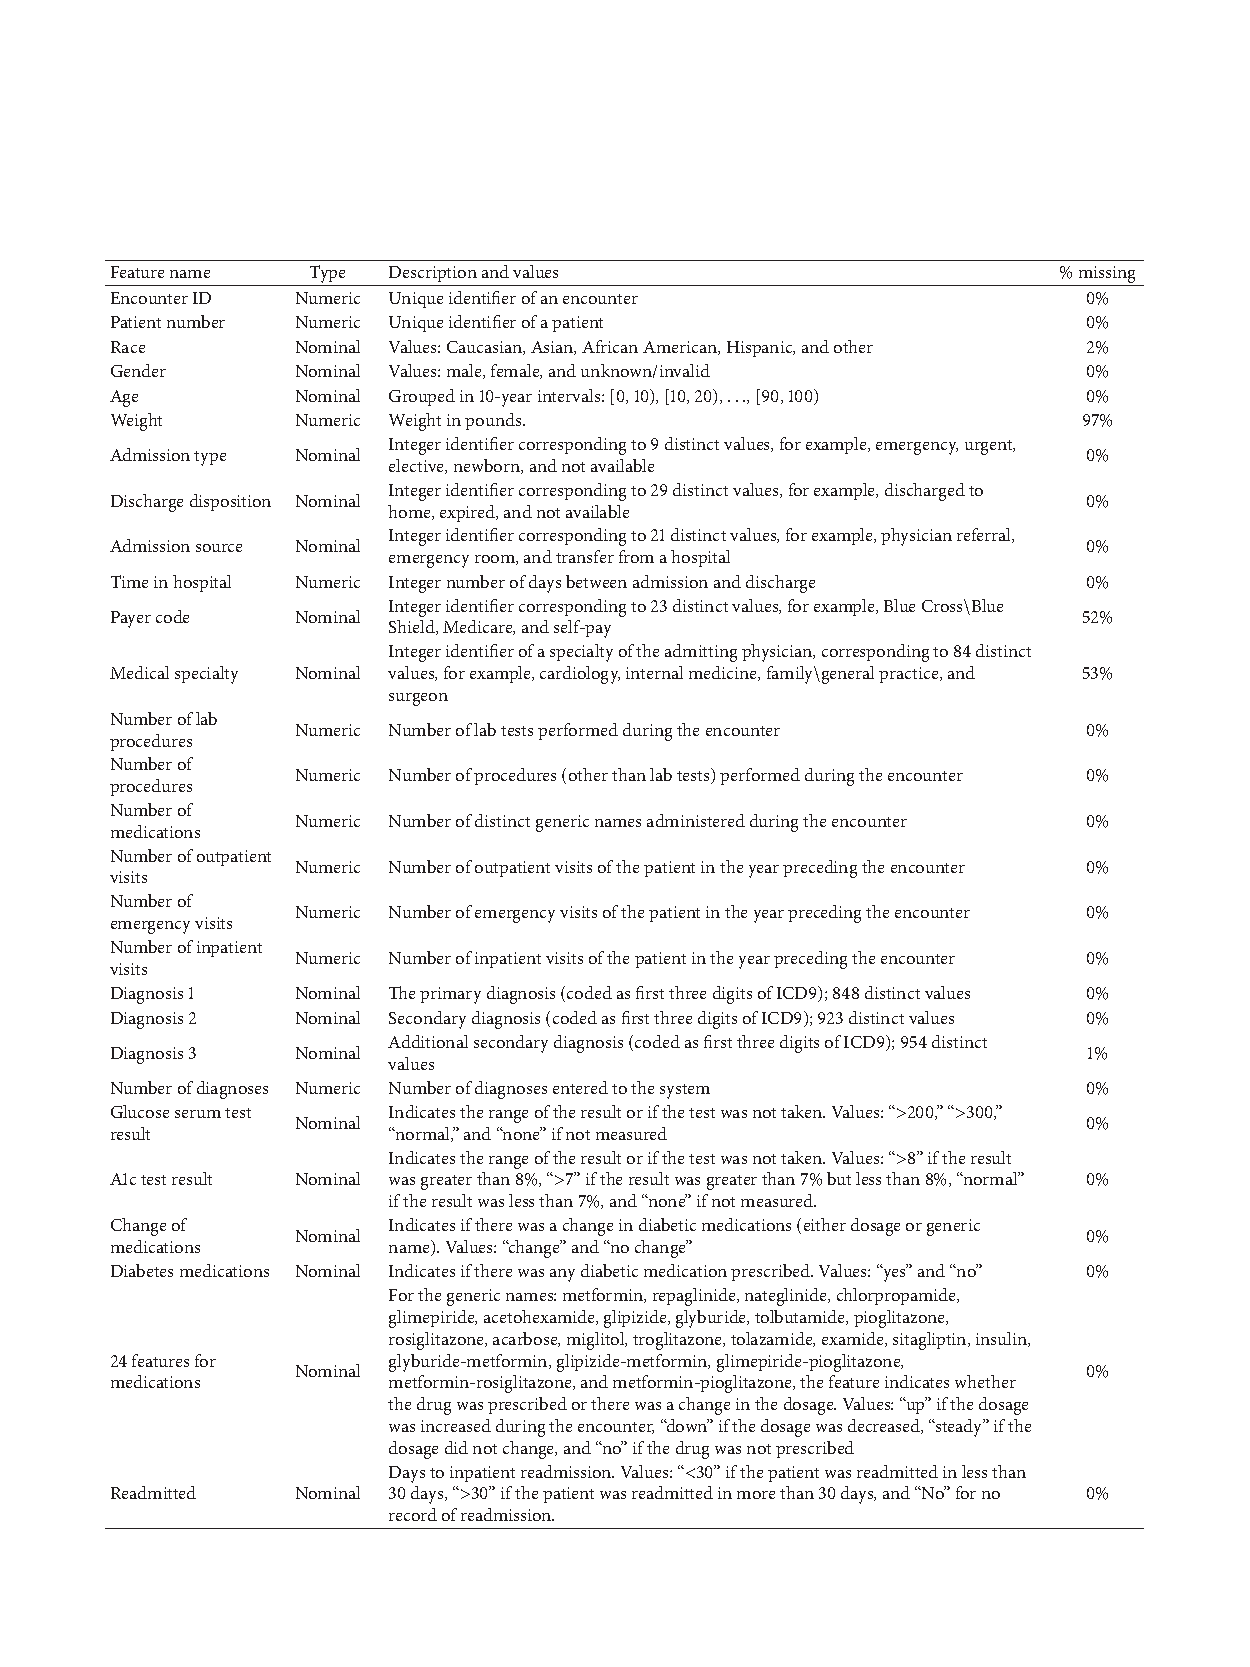
\includegraphics[width=15cm]{features.pdf}
    \label{features}
\end{table}

This dataset contains a set of 55 features, selected by clinical experts and described in Table \ref{features}, potentially associated with the diabetic condition or management. \\
The readmission attribute we are interested in has been redefined into two values: "readmitted" if the patient was readmitted within 30 days of discharge or "otherwise", which covers both readmission after 30 days and no readmission at all.

The measurement of the Hemoglobin A1c (HbA1c) gives important indication of the glucose control and it is widely applied to measure performance of diabetes care [4, 5]. The measurement of HbA1c at the time of hospital admission offers a unique opportunity to assess the efficacy of current therapy and to make changes in that therapy if indicated (e.g., HbA1c $>$ 8.0$\%$ on current regimen).
The attribute "A1c test result" indicates if the test was done or not and if yes gives the range of the result. 
Both the frequency of HbA1c test ordering and the response to its result, which is defined as a change in diabetic medications (any dosage change (increase or reduction) as well as change to a drug with a different generic name), were examined. 

We consider four groups of encounters: (1) no HbA1c test performed, (2) HbA1c performed and in normal range, (3) HbA1c performed and the result is greater than 8$\%$ with no change in diabetic medications, and (4) HbA1c performed, result is greater than 8$\%$, and diabetic medication was changed.

\subsection{Data Selection}

The initial dataset described before contains incomplete, redundant and noisy information as expected in any real-world data. Several features has been discarded due to high percentage of missing values such as the weight (97$\%$) and the payer code (40$\%$), the medical specialty of the admitting physician was maintained even with 47$\%$ of missing values.
In the dataset there are multiple inpatient visits for some patient and the observations could not be considered as statistically independent, therefore we kept only encounter per patient. In particular we maintained only the first encounter for each patient as the primary admission and then determined whether or not they were readmitted within 30 days.
In addition all encounters that resulted in either discharge to a hospice or patient death were removed in order to avoid biasing the analysis. \\
After the above-described requirements 69774 encounters are left in the dataset. To summarize, the dataset consists of hospital admissions of length between one and 14 days that did not result in a patient death or discharge to a hospice. Each encounter corresponds to a unique patient diagnosed with diabetes, although the primary diagnosis may be different. During each of the analyzed encounters, lab tests were ordered and medication was administered.

Distributions of some the demographic and illness severity variables in the dataset are shown in Figures \ref{time}, \ref{gender_test} an \ref{med_spec}.

\begin{figure}[t!]
	\hspace{-0.45cm}
    \begin{subfigure}[b]{0.5\textwidth}
    	\hspace{-.5cm}
        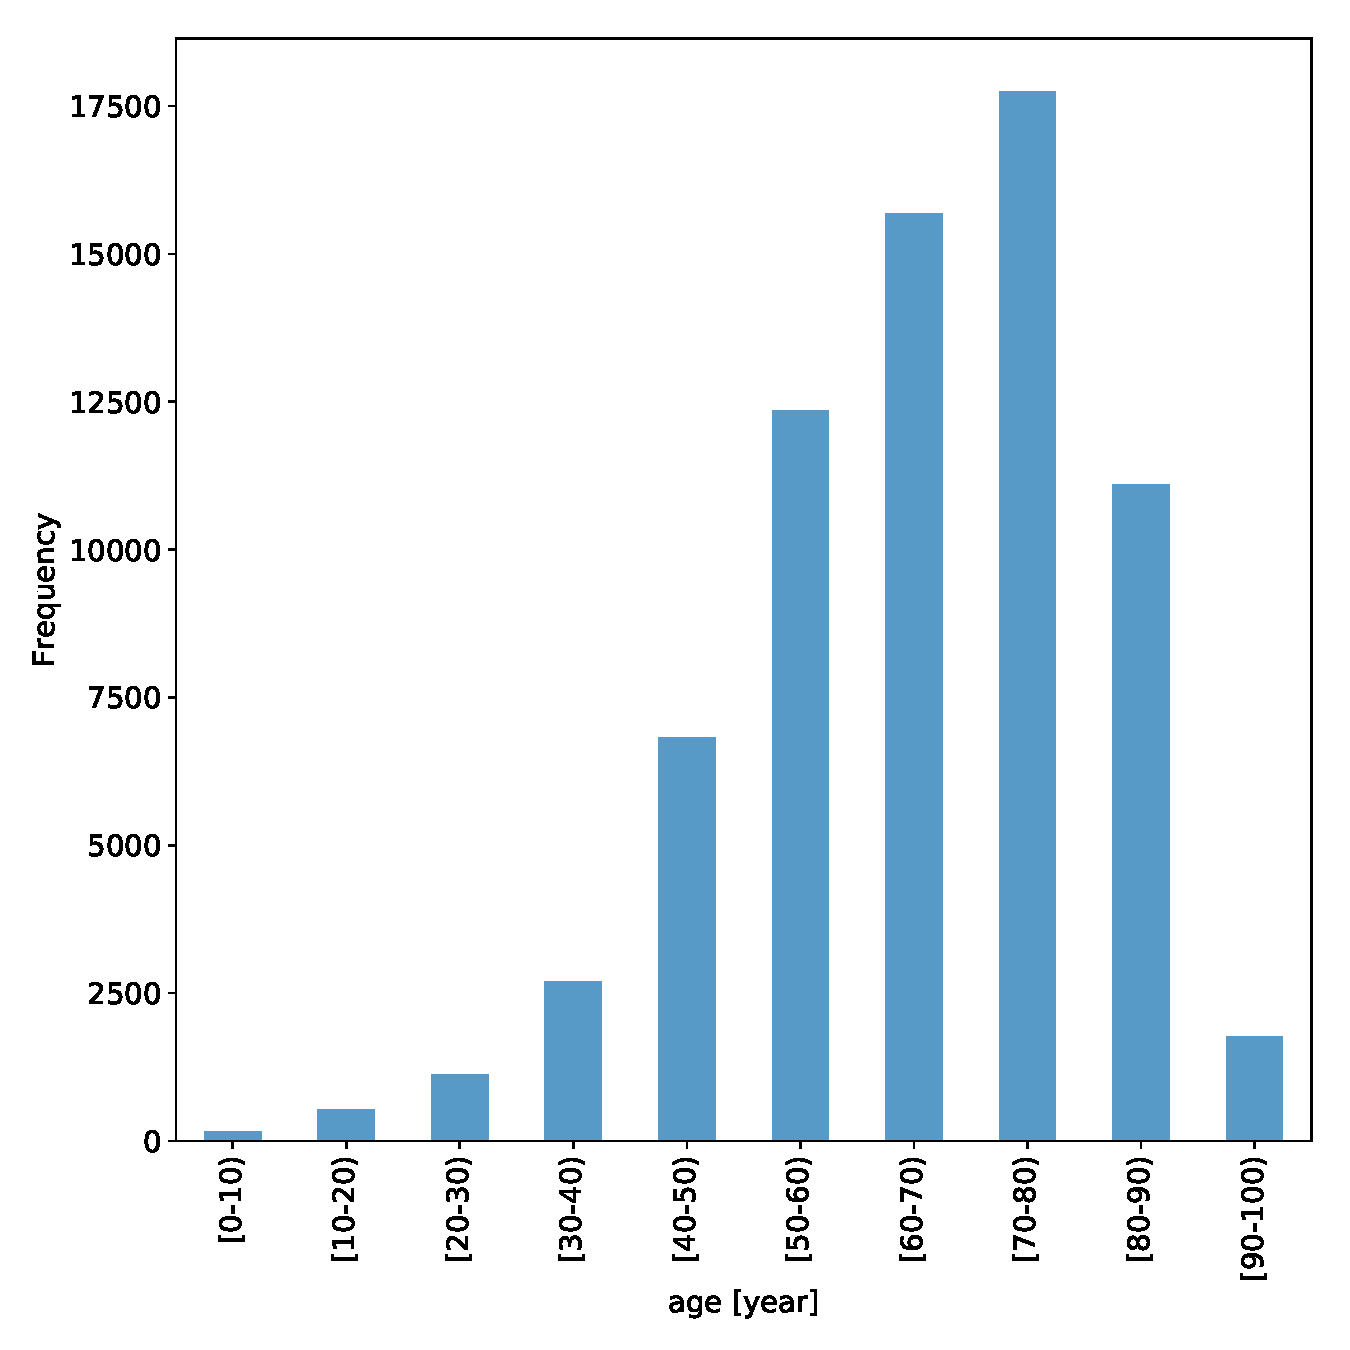
\includegraphics[width=7.8cm]{age.pdf}
        %\caption{}
        \label{fig:chi_FD}
    \end{subfigure}
    \hspace{0.75cm} %add desired spacing between images, e. g. ~, \quad, \qquad, \hfill etc. 
      %(or a blank line to force the subfigure onto a new line)
    \begin{subfigure}[b]{0.5\textwidth}
    	\hspace{-0.5cm}
    	\vspace{+0.47cm}
        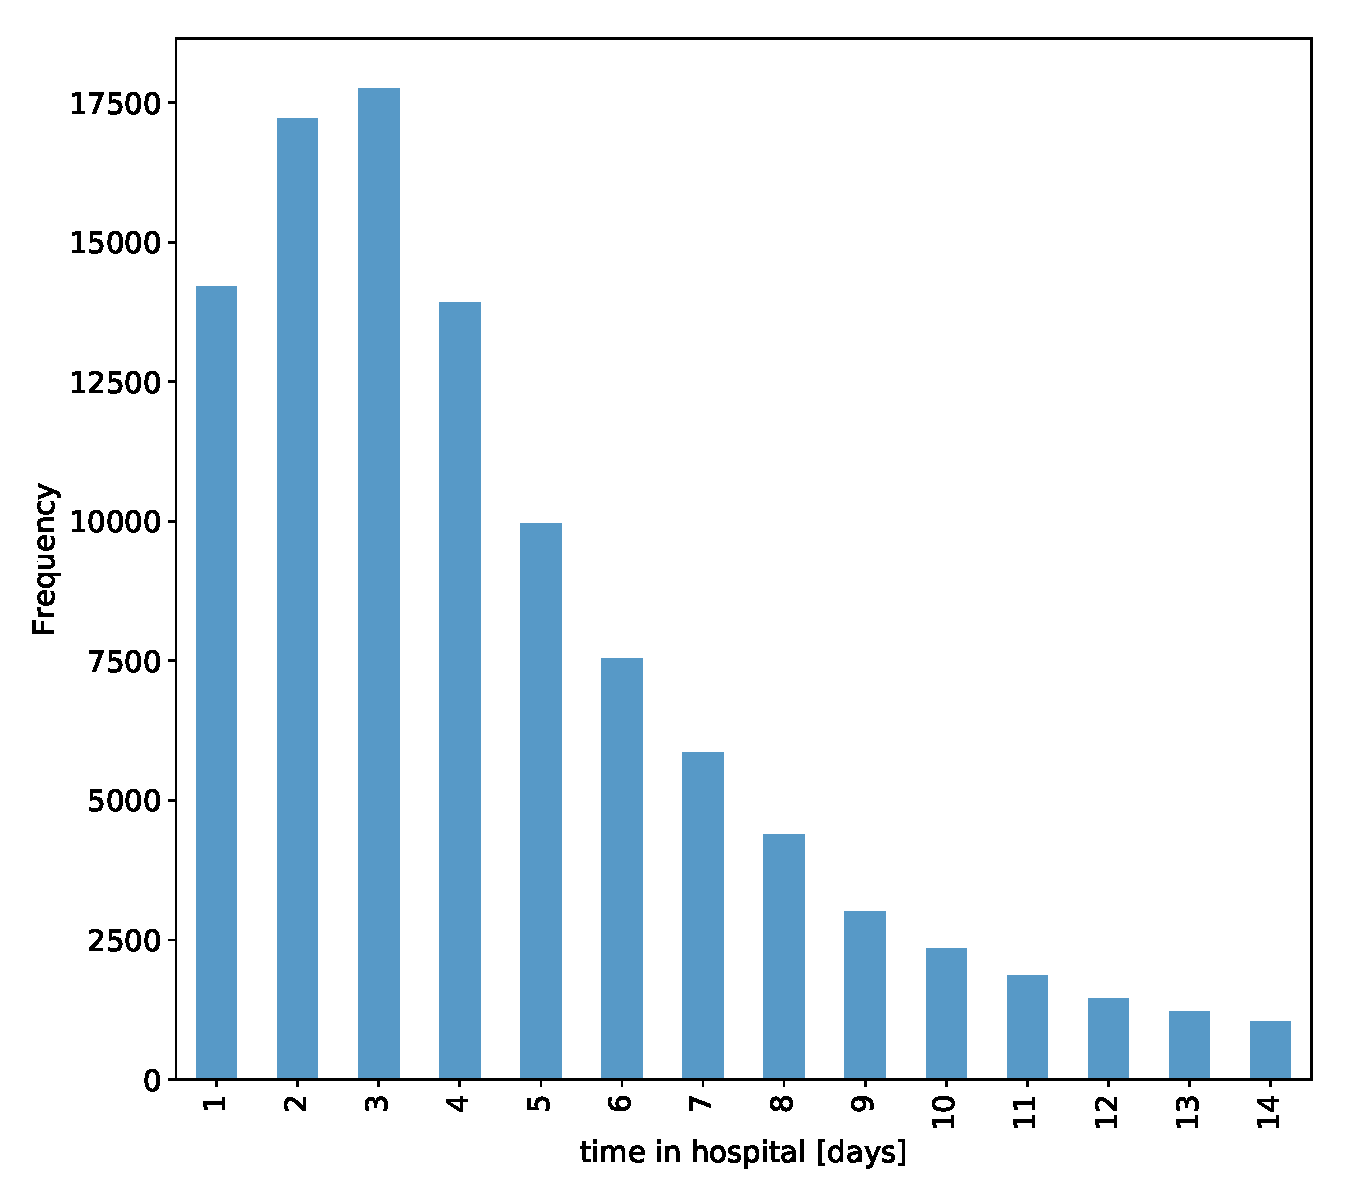
\includegraphics[width=8.2cm]{time_in_hospital.pdf}
        %\caption{misidentified pion}
        \label{fig:chi_Dz}
    \end{subfigure}    

   \caption{\small Age distribution and distribution of the time spent in the hospital of the patients.}
    \label{time}
\end{figure}

\begin{figure}[t!]
	\hspace{-0.7cm}
    \begin{subfigure}[b]{0.5\textwidth}
    	\hspace{-.5cm}
        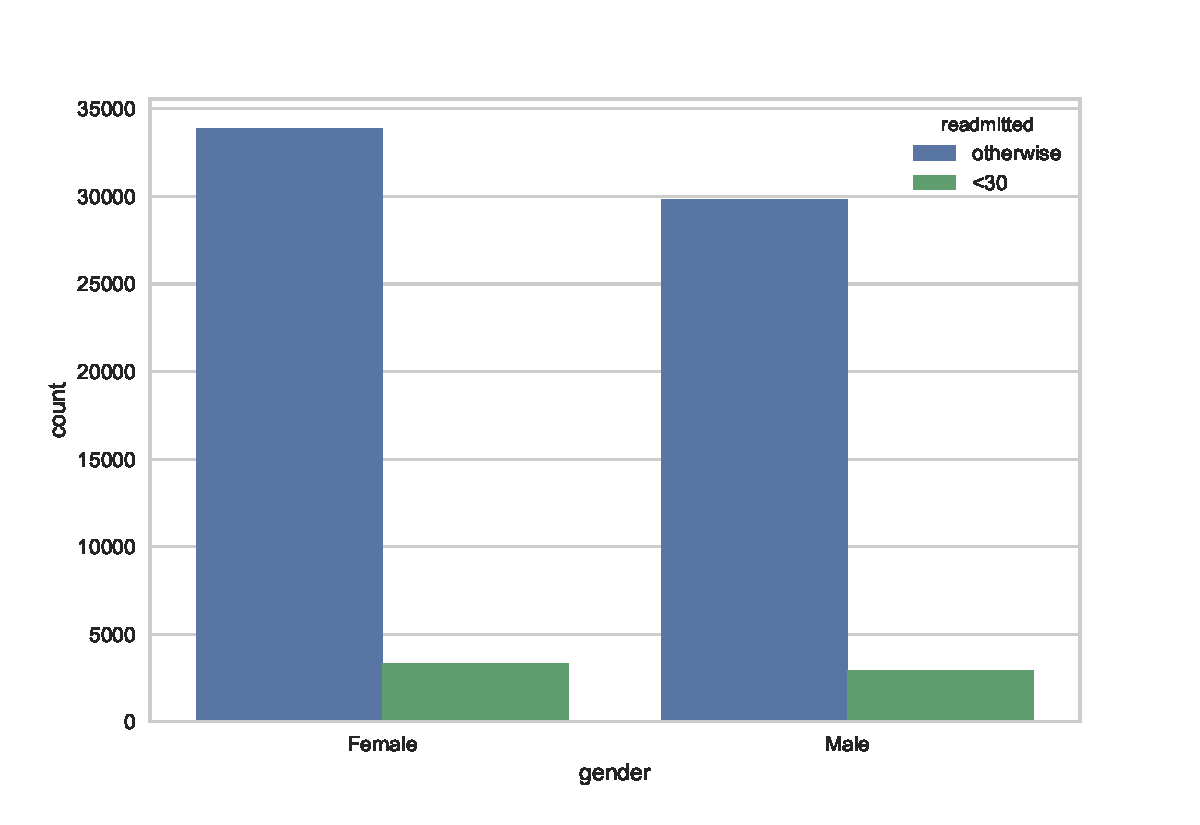
\includegraphics[width=9.2cm]{gender.pdf}
        %\caption{}
        \label{fig:chi_FD}
    \end{subfigure}
    \hspace{0.8cm} %add desired spacing between images, e. g. ~, \quad, \qquad, \hfill etc. 
      %(or a blank line to force the subfigure onto a new line)
    \begin{subfigure}[b]{0.5\textwidth}
    	\hspace{-0.5cm}
    	%\vspace{+0.47cm}
        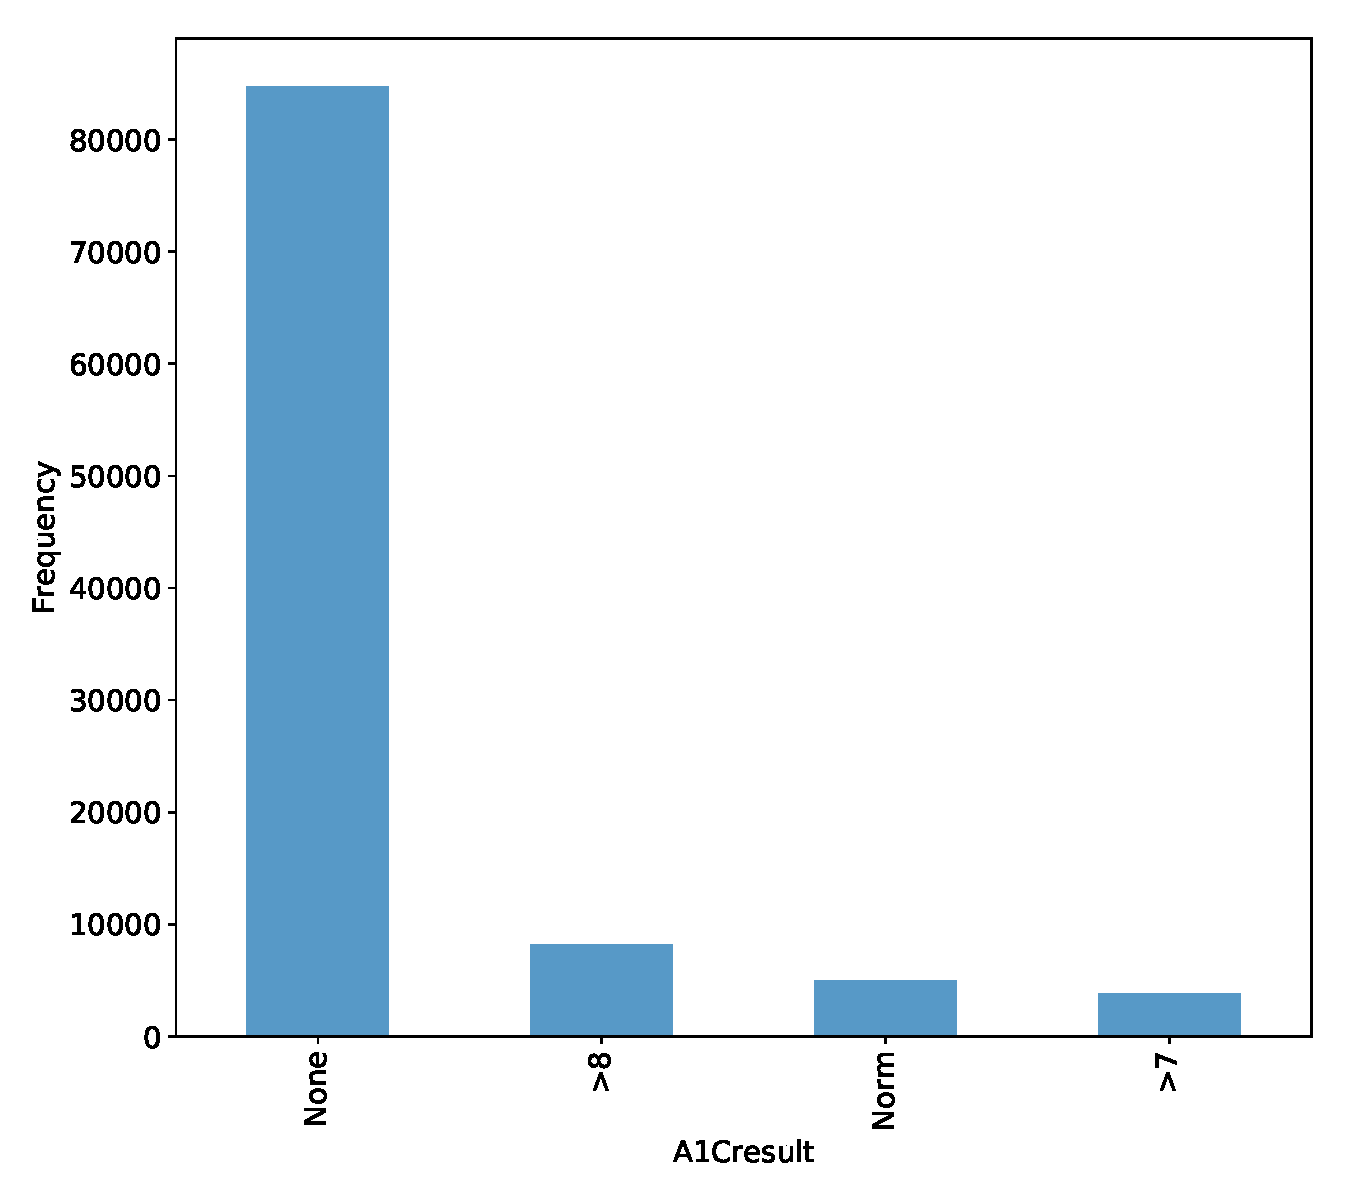
\includegraphics[width=9.2cm]{A1Cresult.pdf}
        %\caption{misidentified pion}
        \label{fig:chi_Dz}
    \end{subfigure}    

   \caption{\small Distributions of patients races and A1C tests in the case the patients are readmitted within 30 (green) days or not (blue).}
    \label{gender_test}
\end{figure}

\begin{figure}[t!]
   \centering
    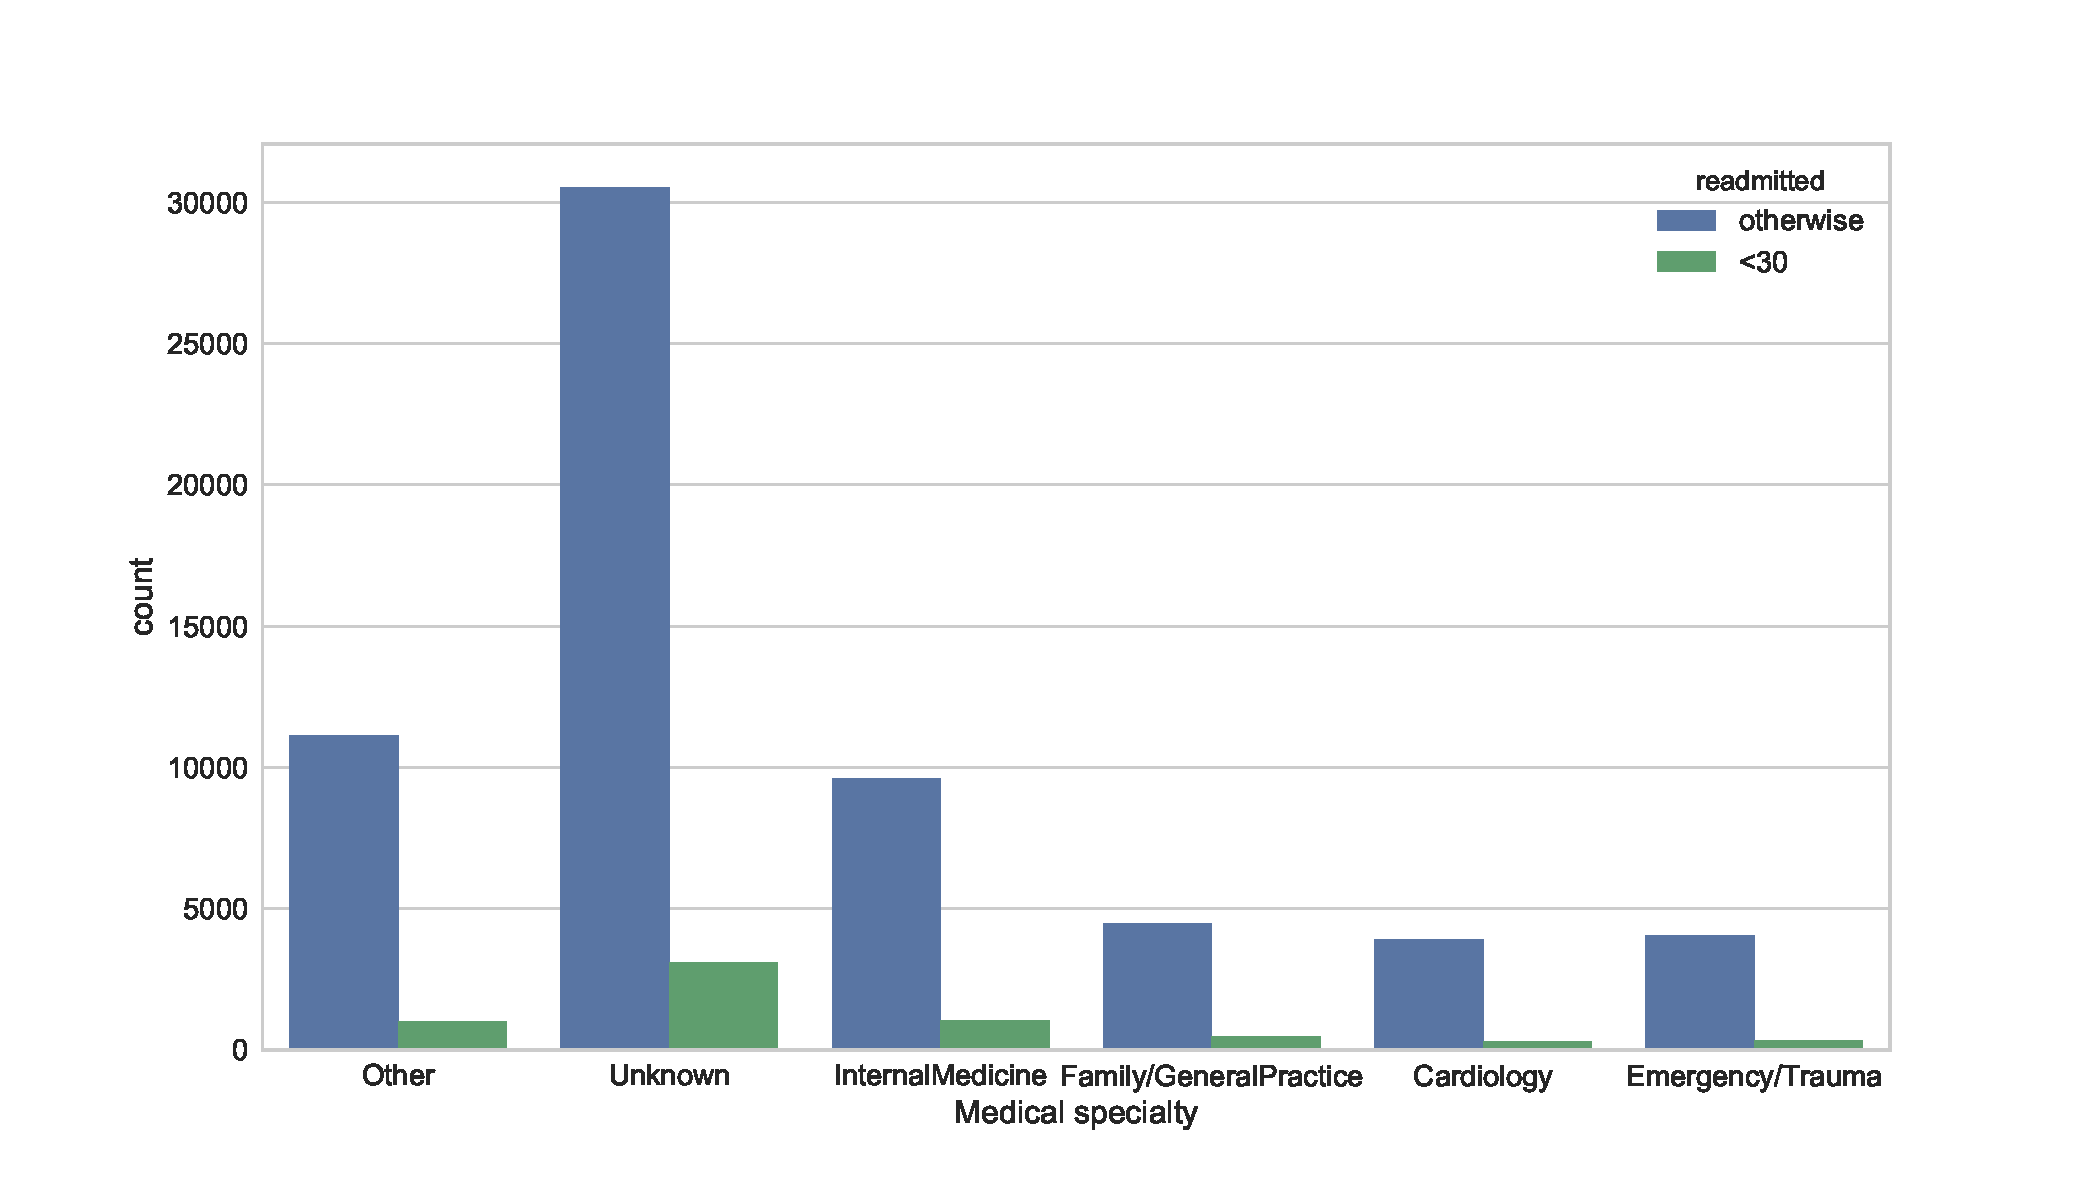
\includegraphics[width=16cm]{med_spec.pdf}
    \caption{\small Specialty of the admitting physician distribution in case the case the patients are readmitted within 30 days (green) or not (blue). }
    \label{med_spec}
\end{figure}

All values of the diagnosis features have been grouped into categories, the Table \ref{diag}  shows these categories for the first diagnosis and and their distributions in the dataset.

\subsection{Strategy}

Multivariate logistic regression, random decision forests and gradient boosting classification from scikit-learn are used to fit the relationship between the measurement of HbA1c and early readmission.
As we are dealing with a lot of categorical (some with high cardinality) and numerical features several assumptions and requirements have been done in order to reduce the number of features. The number of medical specialties is reduced in order to keep only the most significant ones (the rest is grouped under an "Other" category), a threshold on the number of encounters is set for the types of admissions and discharge dispositions (encounters under this threshold are put in an "Other" category) and finally the 24 diabetes medications features are hashed into a lower number of outputs; all of  these requirements will be optimized.



\begin{table}[t!]
   \centering
    \caption{\small Values of the primary diagnosis in the final dataset. In the analysis, groups that covered less than 3.5$\%$ of encounters were grouped into "other" category.}
    \vspace{0.2cm}
    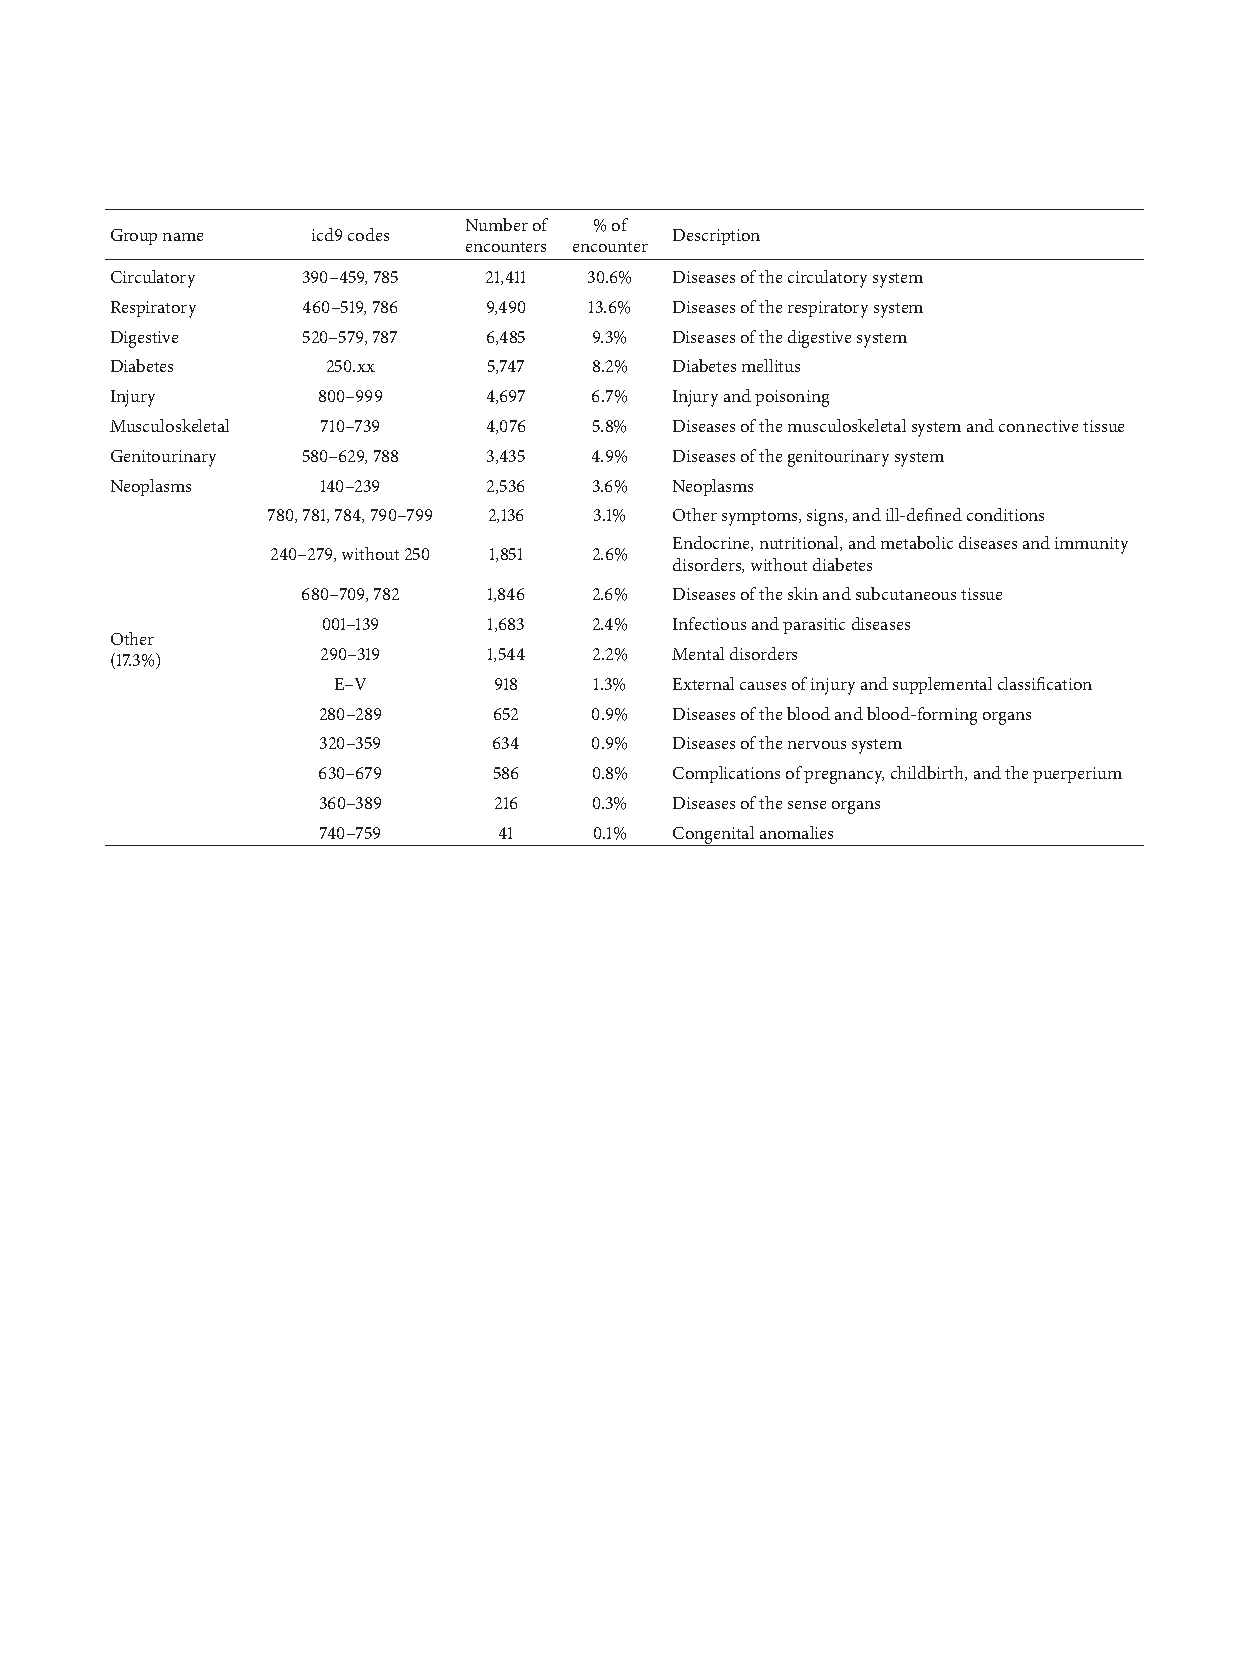
\includegraphics[width=15cm]{diag.pdf}
    \label{diag}
\end{table}

\section{Results and Discussion}

A primary analysis has been done using logistic regression. The requirements to reduce the number of features have been optimized using this classifier and results in keeping only 7 medical specialties, a threshold of 100 encounters for types of admission and 500 for types of discharge disposition. Finally the diabetes medications have been hashed into 8 outputs.

\begin{figure}[t!]
   \centering
    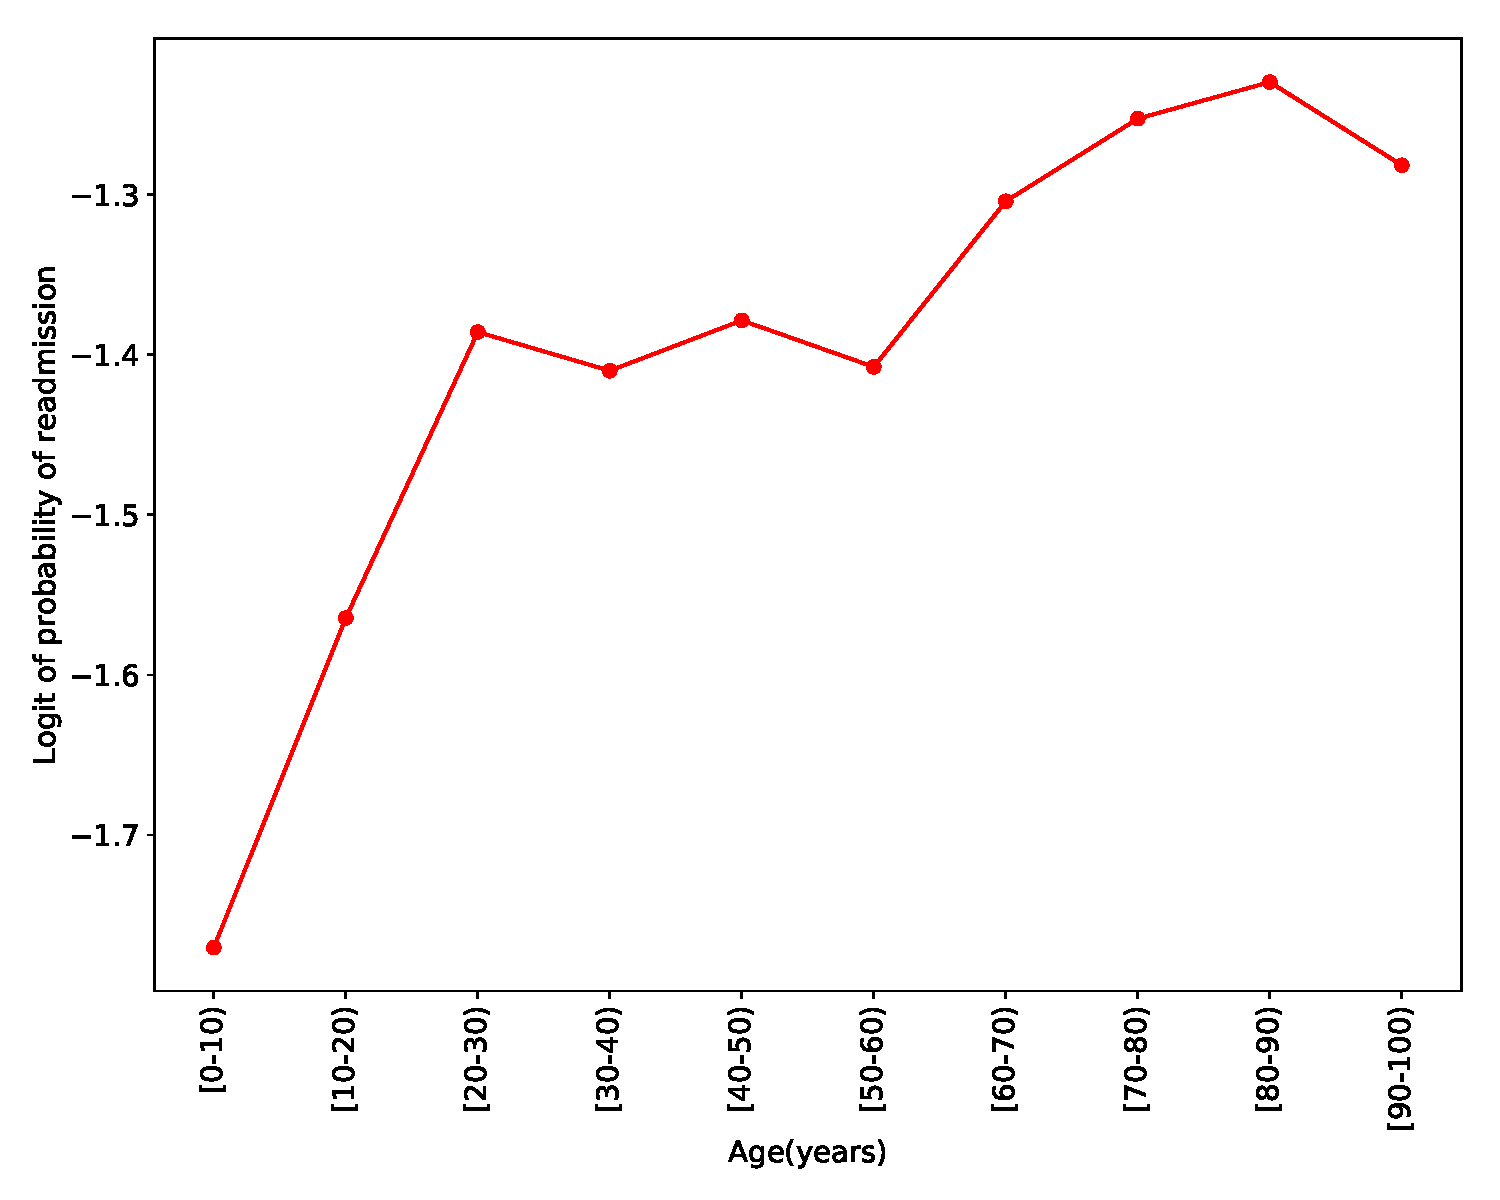
\includegraphics[width=11cm]{age_logit.pdf}
    \caption{\small Relationship of age and the logistic function of the readmission rate. }
    \label{logit_age}
\end{figure}

Fig. \ref{logit_age} shows that we can divide the age feature into three groups, indeed there are three regimes for the logit of probability of readmission rate. For the next steps we can defined three ages categories from 0 to 20 year, from 20 to 60 years and from 60 to 100 years. 

Logistic regression, random forest decision and gradient boosting classifier have been trained on this newly defined dataset and the gender feature has been discarded from the dataset due to a poor significance for those classifiers. All classifiers are able to predict if a patient was readmitted within 30 days with an accuracy of 91$\%$.


Fig. \ref{prob_A1c} shows the probability of readmission estimated from the three classifiers for the four groups of encounters
defined in Section \ref{init} for encounters being primary diagnosed to have a diabetes, circulatory or respiratory issue. We see observe a decrease of the probability of readmission for patient diagnosed with diabetes when a HbA1c test is done will all classifiers.
 
 


\begin{figure}[t!]
   \centering
    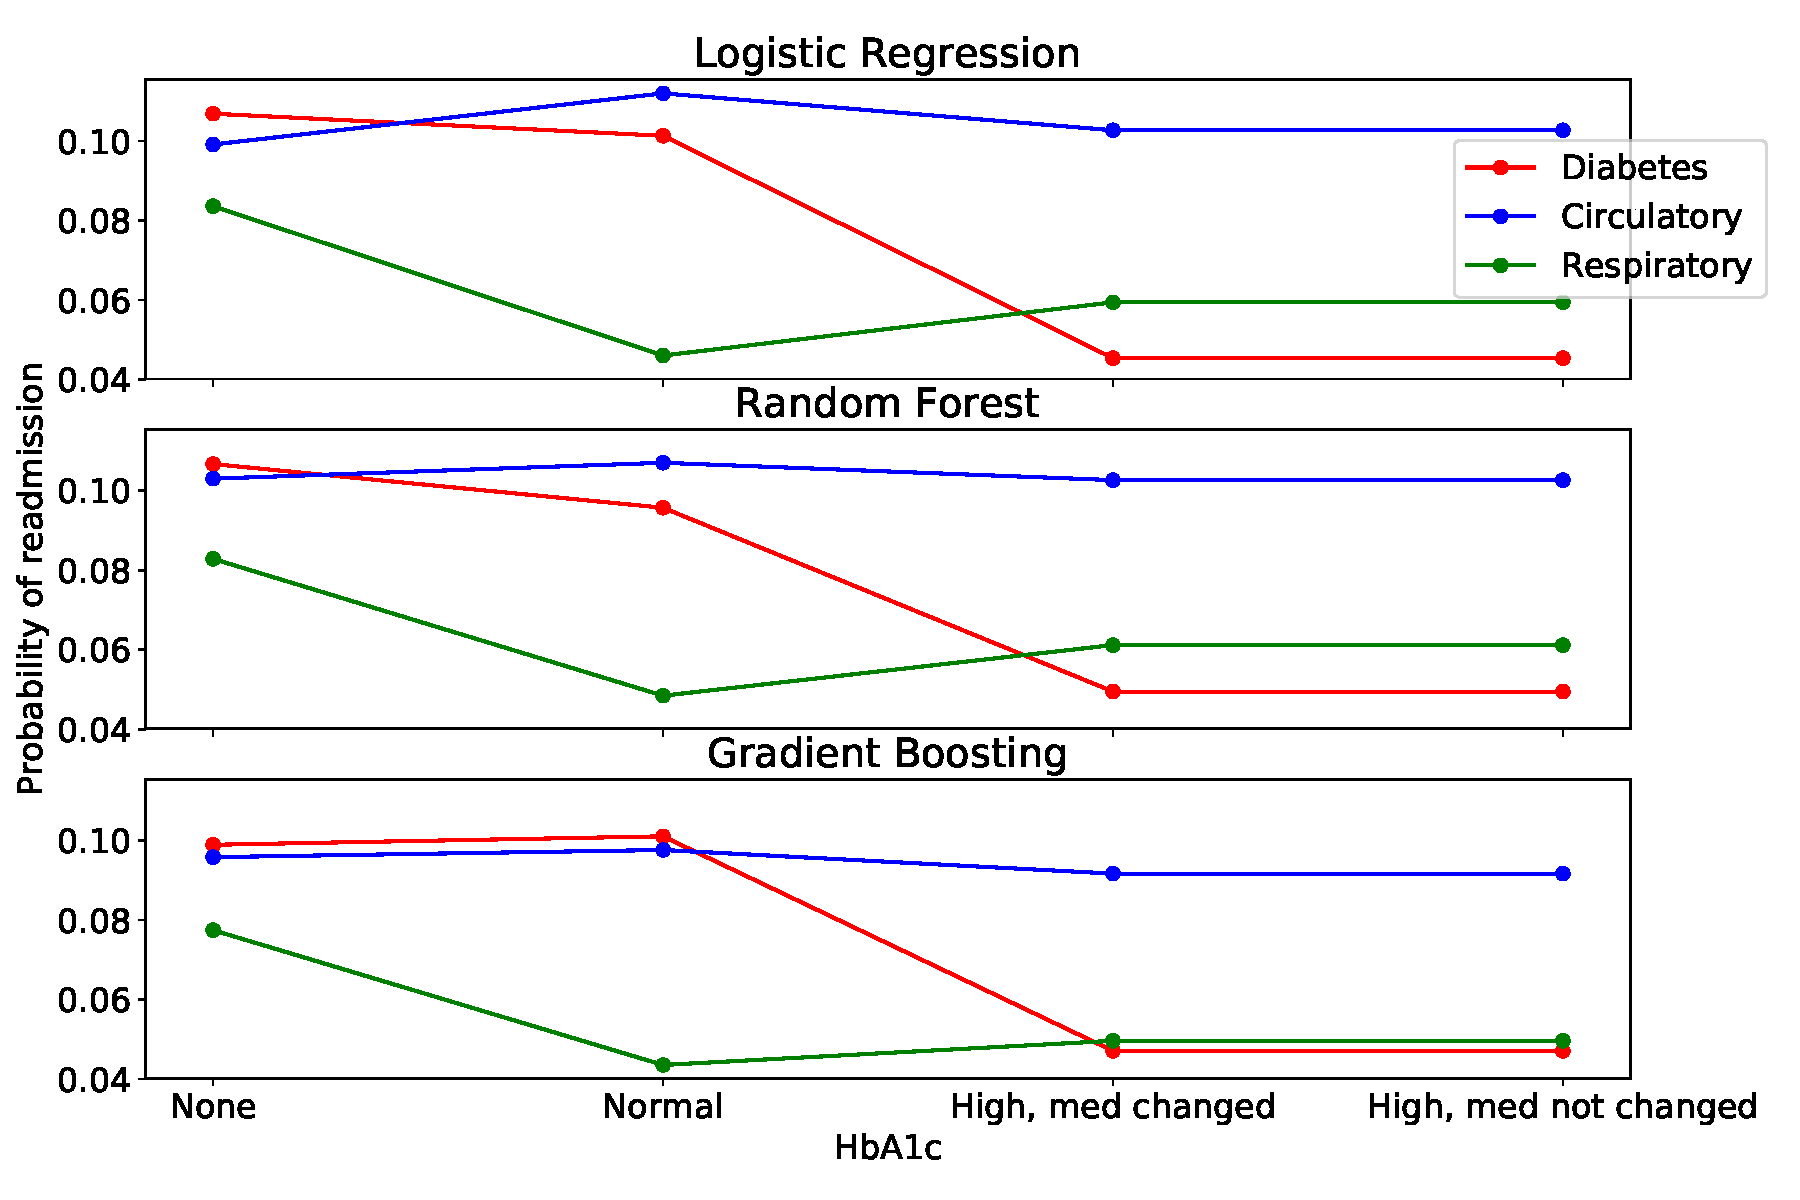
\includegraphics[width=14cm]{prob_A1c.pdf}
    \caption{\small Readmission rates for the four groups of encounters described in Section \ref{init} and for different primary diagnosis (Diabetes, Respiratory and Circulatory). }
    \label{prob_A1c}
\end{figure}

\section{Conclusion}

The hypothesis that the measurement of the hemoglobin A1c is associated with a reduction in readmission rates has been shown to be true.  HbA1c is therefore a useful predictor of readmission rates which might be valuable in the development of strategies to reduce readmission rates and costs for the care of individuals with diabetes mellitus.
The analysis also shown that the profile of readmission differed  significantly for patients where HbA1c was checked in the setting of a primary diabetes diagnosis compared to patients with a primary circulatory disorder (for which the readmission rates are the highest). It seems the readmission rates for patient with diabetes is associated with the decision to test for HbA1c but not if diabetes medications were changed or not..


% Your references go at the end of the main text, and before the
% figures.  For this document we've used BibTeX, the .bib file
% scibib.bib, and the .bst file Science.bst.  The package scicite.sty
% was included to format the reference numbers according to *Science*
% style.

\subsection*{References}
\begin{itemize}
\item[1.]
Beata Strack, Jonathan P. DeShazo, Chris Gennings, \textit{et al}., "Impact of HbA1c Measurement on Hospital Readmission Rates: Analysis of 70,000 Clinical Database Patient Records," \textit{BioMed Research International}, vol. 2014, Article ID 781670, 11 pages, 2014. doi:10.1155/2014/781670
\item[2.]
Scikit-learn: Machine Learning in Python, Pedregosa \textit{et al}., JMLR 12, pp. 2825-2830, 2011
\item[3.]
A. Frank and A. Asuncion, \textit{UCI Machine Learning Repository}, University of California, School of Information and Computer Science, 2010.
\item[4.]
D. Baldwin, G. Villanueva, R. McNutt, and S. Bhatnagar, "Eliminating inpatient sliding-scale insulin: a reeducation project with medical house staff," \textit{Diabetes Care}, vol. 28, no. 5, pp. 1008?1011, 2005.
\item[5.]
H. Anwar, C. M. Fischbacher, G. P. Leese \textit{et al}., "Assessment of the under-reporting of diabetes in hospital admission data: a study from the Scottish diabetes research network epidemiology group," \textit{Diabetic Medicine}, vol. 28, no. 12, pp. 1514?1519, 2011.
\end{itemize} 


\bibliography{scibib}


\bibliographystyle{Science}



% Following is a new environment, {scilastnote}, that's defined in the
% preamble and that allows authors to add a reference at the end of the
% list that's not signaled in the text; such references are used in
% *Science* for acknowledgments of funding, help, etc.





% For your review copy (i.e., the file you initially send in for
% evaluation), you can use the {figure} environment and the
% \includegraphics command to stream your figures into the text, placing
% all figures at the end.  For the final, revised manuscript for
% acceptance and production, however, PostScript or other graphics
% should not be streamed into your compliled file.  Instead, set
% captions as simple paragraphs (with a \noindent tag), setting them
% off from the rest of the text with a \clearpage as shown  below, and
% submit figures as separate files according to the Art Department's
% instructions.


\clearpage


\end{document}




















